\documentclass[a4paper, 10pt, twoside]{article}

\usepackage[top=1in, bottom=1in, left=1in, right=1in]{geometry}
\usepackage[utf8]{inputenc}
\usepackage[spanish, es-ucroman, es-noquoting]{babel}
\usepackage{setspace}
\usepackage{fancyhdr}
\usepackage{lastpage}
\usepackage{amsmath}
\usepackage{amsfonts}
\usepackage{amsthm}
\usepackage{verbatim}
\usepackage{fancyvrb}
\usepackage{graphicx}
\usepackage{float}
\usepackage{enumitem} % Provee macro \setlist
\usepackage{tabularx}
\usepackage{multirow}
\usepackage{hyperref}
\usepackage{xspace}
\usepackage{qtree}
\usepackage[toc, page]{appendix}


%%%%%%%%%% Constantes - Inicio %%%%%%%%%%
\newcommand{\titulo}{Trabajo Práctico 2}
\newcommand{\materia}{Ingeniería de Software II}
\newcommand{\integrantes}{Izcovich · Lovisolo · Petaccio · Vita}
\newcommand{\cuatrimestre}{Primer Cuatrimestre de 2015}
%%%%%%%%%% Constantes - Fin %%%%%%%%%%


%%%%%%%%%% Configuración de Fancyhdr - Inicio %%%%%%%%%%
\pagestyle{fancy}
\thispagestyle{fancy}
\lhead{\titulo\ · \materia}
\rhead{\integrantes}
\renewcommand{\footrulewidth}{0.4pt}
\cfoot{\thepage /\pageref{LastPage}}

\fancypagestyle{caratula} {
   \fancyhf{}
   \cfoot{\thepage /\pageref{LastPage}}
   \renewcommand{\headrulewidth}{0pt}
   \renewcommand{\footrulewidth}{0pt}
}
%%%%%%%%%% Configuración de Fancyhdr - Fin %%%%%%%%%%


%%%%%%%%%% Miscelánea - Inicio %%%%%%%%%%
% Evita que el documento se estire verticalmente para ocupar el espacio vacío
% en cada página.
\raggedbottom

% Separación entre párrafos.
\setlength{\parskip}{0.5em}

% Separación entre elementos de listas.
\setlist{itemsep=0.5em}

% Asigna la traducción de la palabra 'Appendices'.
\renewcommand{\appendixtocname}{Apéndices}
\renewcommand{\appendixpagename}{Apéndices}

\newcommand{\grafico}[1]{
  \begin{center}
    \includegraphics[width=15cm]{#1}
  \end{center}
}

\newcommand{\riesgo}[7]{
  \underline{Riesgo {#1}:}
  \begin{itemize}   
    \item \textbf{Descripción:} {#2}
    \item \textbf{Probablidad:} {#3}
    \item \textbf{Impacto:} {#4}
    \item \textbf{Exposición:} {#5}
    \item \textbf{Mitigación:} {#6}
    \item \textbf{Plan de contingencia:} {#7}
  \end{itemize}
}

\newcommand{\escenario}[7] {
  \textit{{#1}}
  \begin{itemize}
    \item \textbf{Fuente:} {#2}
    \item \textbf{Estímulo:} {#3}
    \item \textbf{Entorno:} {#4}
    \item \textbf{Artefacto:} {#5}
    \item \textbf{Respuesta:} {#6}
    \item \textbf{Medición:} {#7}
  \end{itemize}
}

%%%%%%%%%% Miscelánea - Fin %%%%%%%%%%

\begin{document}


%%%%%%%%%%%%%%%%%%%%%%%%%%%%%%%%%%%%%%%%%%%%%%%%%%%%%%%%%%%%%%%%%%%%%%%%%%%%%%%
%% Carátula                                                                  %%
%%%%%%%%%%%%%%%%%%%%%%%%%%%%%%%%%%%%%%%%%%%%%%%%%%%%%%%%%%%%%%%%%%%%%%%%%%%%%%%


\thispagestyle{caratula}

\begin{center}


\includegraphics[height=2cm]{DC.png} 
\hfill

\includegraphics[height=2cm]{UBA.jpg} 

\vspace{2cm}

Departamento de Computación,\\
Facultad de Ciencias Exactas y Naturales,\\
Universidad de Buenos Aires

\vspace{4cm}

\begin{Huge}
\titulo
\end{Huge}

\vspace{0.5cm}

\begin{Large}
\materia
\end{Large}

\vspace{1cm}

\cuatrimestre

\vspace{4cm}

\begin{tabular}{|c|c|c|}
\hline
Apellido y Nombre & LU & E-mail\\
\hline
Izcovich, Sabrina      & 550/11 & sizcovich@gmail.com\\
Lovisolo, Leandro      & 645/11 & leandro@leandro.me\\
Petaccio, Lautaro José & 443/11 & lausuper@gmail.com\\
Vita, Sebastián        & 149/11 & sebastian\_vita@yahoo.com.ar\\
\hline
\end{tabular}

\end{center}

\newpage

\tableofcontents

\newpage


%%%%%%%%%%%%%%%%%%%%%%%%%%%%%%%%%%%%%%%%%%%%%%%%%%%%%%%%%%%%%%%%%%%%%%%%%%%%%%%
%% Introducción                                                              %%
%%%%%%%%%%%%%%%%%%%%%%%%%%%%%%%%%%%%%%%%%%%%%%%%%%%%%%%%%%%%%%%%%%%%%%%%%%%%%%%

\section{Introducción}

En el presente trabajo se aborda la extensión del diseño presentado en el TP1, debiendo ahora plantear un sistema de mensajes de muchas campañas a nivel nacional tanto para servicios públicos como privados. Dada esta nueva situación, aparecen varios stakeholders que, por su colaboración en el proyecto proveyendo servicios, o por su intención de consumo, imponen distintos requerimientos que sumados a los técnicos desembocan en la contemplación de diversos riesgos y atributos de calidad.
Aquí se presenta una planificación de las fases de elaboración, construcción y transición de la metodología UP, asumiendo que la fase inception ya se ha desarrollado. En esta primera etapa se presentan las ideas para la formulación del proyecto Big Tiza, se establecen los requerimientos y recursos disponibles, y se lleva a cabo el QAW del cual se desprendieron algunos atributos de calidad esperados en el producto final. Como parte de la primera iteración, se identifican los casos de uso más relevantes y en base a la recopilación de toda esta información se realiza un análisis de riesgos que se utiliza en parte para la organización de los CU en las distintas iteraciones incrementales. Además se diseña la arquitectura del sistema.

\newpage

%%%%%%%%%%%%%%%%%%%%%%%%%%%%%%%%%%%%%%%%%%%%%%%%%%%%%%%%%%%%%%%%%%%%%%%%%%%%%%%
%% Casos de uso                                                              %%
%%%%%%%%%%%%%%%%%%%%%%%%%%%%%%%%%%%%%%%%%%%%%%%%%%%%%%%%%%%%%%%%%%%%%%%%%%%%%%%

\section{Casos de uso}
Para comenzar a trabajar sobre la planificación del proyecto se identificó un conjunto de casos de uso que cubren la mayoría de las funcionalidades que se desprenden de los requerimientos obtenidos. En un principio se los agrupó, tal y como se muestra a continuación, por su funcionalidad. Posteriormente, y en base al análisis de riesgos y a la información destilada de la fase de incepción, se utilizó este refinamiento para la organización y planificación de las iteraciones de elaboración y construcción.

\begin{itemize}

\item \textbf{Comunicación}
\begin{itemize}
\item Enviando mensajes de campañas por medios seleccionados\footnote{Facebook, Twitter, Whatsapp o SMS.}.
\item Respondiendo mensaje a una pregunta.
\end{itemize}

\item \textbf{Monitoreo}
\begin{itemize}
\item Consultando estado de una campaña.
\item Visualizando el mapa de evolución de las campañas.
\end{itemize}

\item \textbf{Auditoría}
\begin{itemize}
\item Registrando cantidad de mensajes enviados por campaña.
\item Generando factura mensual para la empresa de infraestructura privada.
\end{itemize}

\item \textbf{Gestión}
\begin{itemize}
\item Ingresando los resultados de una campaña.
\item Creando, editando y eliminando grupos de destinatarios.
\item Creando una campaña desde el sector público/privado.
\item Desuscribiendo a un destinatario de una campaña.
%\item Reinscribiendo a un destinatario en una campaña de la que se desuscribió.
\item Agregando evaluación manual del resultado de las preguntas.
\item Aceptando campaña privada.
\item Creando cuestionario de campañas de evaluación de campañas.
\item Agregando nuevo usuario proveedor de contenidos.
\item Creando, editando y eliminando usuarios.
\end{itemize}

\item \textbf{Supervisión}
\begin{itemize}
\item Supervisando campañas privadas (supervisar encuestas)?
\item Pidiendo reportes de resultados de una campaña
\item Reportando información anonimizada de grupos de destinatarios.
\end{itemize}

\item \textbf{Seguridad}
\begin{itemize}
\item Autenticando usuario.
\item Guardando datos cifrados en servidores locales.
\end{itemize}
\end{itemize}

\newpage

%%%%%%%%%%%%%%%%%%%%%%%%%%%%%%%%%%%%%%%%%%%%%%%%%%%%%%%%%%%%%%%%%%%%%%%%%%%%%%%
%% Planificación                                                          %%
%%%%%%%%%%%%%%%%%%%%%%%%%%%%%%%%%%%%%%%%%%%%%%%%%%%%%%%%%%%%%%%%%%%%%%%%%%%%%%%

\section{Planificación}

\subsection{Iteraciones}
La división de los CU en las distintas iteraciones y la organización de las mismas estuvo pautada por las necesidades manifestadas por los stakeholders, el análisis de riesgo y un incremento de funcionalidad, partiendo del núcleo más importante y revistiendo la aplicación a lo largo del tiempo de lógica menos prioritaria.

\subsubsection{Fase de iniciación}
Consideramos fase de iniciación al trabajo realizado en el Primer Trabajo Práctico junto con la Arquitectura presente en este TP.

\subsubsection{Fase de elaboración}

\textbf{Primera iteración} [3 semanas]
\begin{enumerate}
\item Guardando datos cifrados en servidores locales.
\item Creando una campaña desde el sector público/privado.
\item Enviando mensajes de campañas por medios seleccionados.
\item Autenticando usuario.
\end{enumerate}

\textbf{Segunda iteración} [5 semanas]
\begin{enumerate}
\item Creando, editando y eliminando usuarios.
\item Consultando estado de una campaña.
\item Registrando cantidad de mensajes enviados por campaña.
\item Creando, editando y eliminando grupos de destinatarios.
\end{enumerate}

\textbf{Tercera iteración} [5 semanas]
\begin{enumerate}
\item Creando cuestionario de campañas de evaluación de campañas.
\item Respondiendo mensaje a una pregunta.
\item Desuscribiendo a un destinatario de una campaña.
\item Reinscribiendo a un destinatario en una campaña de la que se desuscribió.
\end{enumerate}

\textbf{Cuarta iteración} [4 semanas]
\begin{enumerate}
\item Ingresando los resultados de una campaña.
\item Pidiendo reportes de resultados de una campaña.
\item Agregando evaluación manual del resultado de las preguntas.
\end{enumerate}

\textbf{Quinta iteración} [4 semanas]
\begin{enumerate}
\item Aceptando campaña privada.
\item Reportando información anonimizada de grupos de destinatarios.
\item Generando factura mensual para el sector privado.
\item Enviando resultados de campañas a la NSA.
\end{enumerate}

\textbf{Sexta iteración} [4 semanas]
\begin{enumerate}
\item Supervisando campañas privadas (supervisar encuestas).
\item Visualizando el mapa de evolución de las campañas.
\item Agregando nuevo usuario proveedor de contenidos.
\end{enumerate}


\subsection{Alcance de casos de usos de la primera iteración}
\textbf{Guardando datos cifrados en servidores locales.}

Los datos de los usuarios deben almacenarse encriptados en los servidores locales de su región correspondiente para poder garantizar la confidencialidad de los mismos.

Llamamos datos a los registros en la base de datos que contienen información sobre los residentes de la región. Estos pueden ser datos básicos como por ejemplo (nombre, apellido, dni, número de teléfono) y datos adiciones como si es fumador, si poseen un auto, si les gusta correr, etc.

\textbf{Creando una campaña desde el sector público/privado.}

La creación de una campaña consiste en el ingreso de los datos necesarios para la creación de la misma, es decir, un conjunto de mensajes con el horario en el que deben ser enviados, un conjunto de grupos de destinatarios concernientes al objetivo de la campaña y el canal a través del que se enviarán (SMS, Facebook, etc).

\textbf{Enviando mensajes de campañas por medios seleccionados.}

Cada región tiene un sistema de envío de mensajes que periódicamente recorre las campañas asociadas a esa región y envía los mensajes de las mismas cumpliendo su fecha y hora de envío. Además, cada mensaje es enviado por los canales previamente seleccionados a través de la infraestructura propia de cada región.

\textbf{Autenticando usuario.}

Se solicita un usuario y contraseña cuando una persona intenta iniciar una sesión en el sistema para crear una campaña y consultar el estado de una campaña, entre otras. La autenticación también abarca al sector privado dónde tendran acceso sólo a acciones de su sector.

El sistema verifica que las credenciales ingresadas sean válidas, y en caso contrario deniega el acceso al mismo.

\subsection{Tareas CU Primera iteración}
A continuación se detallan las tareas diagramadas para los casos de uso incluidos en la primera iteración con su respectiva estimación de horas hombre.
\\

\begin{tabular}{lp{13cm}l}
  \hline
  CU1 & Guardando datos cifrados en servidores locales & 35h \\
  \hline \\
  T01 & Investigación de fuentes de información disponibles de cada usuario accesible desde el sistema & 4h \\
  T02 & Definición de campos relevantes para almacenar por usuario & 3h \\
  T03 & Diseño de la base de datos & 4h \\
  T04 & Definición de motor de búsqueda a utilizar & 2h \\
  T05 & Definición de método de encriptación & 2h \\
  T06 & Implementación de CU1 & 10h\\
  T07 & Testing de CU1 & 10h \\
  \hline
\end{tabular}

\begin{tabular}{lp{13cm}l}
  \hline
  CU2 & Creando una campaña desde el sector público/privado & 15h \\
  \hline \\
  T01 & Investigar librerías y herramientas para la implementación de las campañas & 5h \\
  T02 & Diseño de la interfaz del usuario & 2h \\
  T03 & Implementación de CU2 & 4h \\
  T04 & Testing de CU2 & 4h \\
  \hline
\end{tabular}

\begin{tabular}{lp{13cm}l}
  \hline
  CU3 &  Enviando mensajes de campañas por medios seleccionados & 40h \\
  \hline \\
  T01 & Investigación de los distintos medios de envío de mensajes & 10h \\
  T02 & Diseño de un servicio EmisorDeMensajes, que en intervalos de tiempo regulares envíe los mensajes programados & 10h \\
  T03 & Implementación de CU3 & 10h \\
  T04 & Testing de CU3 & 10h \\
  \hline
\end{tabular}

\begin{tabular}{lp{13cm}l}
  \hline
  CU4 & Autenticando usuario & 4h \\
  \hline \\
  T01 & Diseño de la interfaz del usuario para autenticación & 1h \\
  T02 & Diseño de los requisitos mínimos de las contraseñas & 1h \\
  T02 & Implementación de CU4 & 1h \\
  T03 & Testing de CU4 & 1h \\
  \hline
\end{tabular}

\subsection{Detalle Primera iteración}
\begin{itemize}
  \item \textbf{Identificación:} E1
  \item \textbf{Tipo de iteración:} Elaboración
  \item \textbf{Cantidad total de horas:} 120
  \item \textbf{Tareas:}
\begin{enumerate}
  \item Refinamiento de objetivos y requerimientos (2h)
  \item Análisis de riesgo (2h)
  \item Reconocimiento de casos de uso (3h)
  \item División de CU en iteraciones según prioridad (1h)
  \item Estimación de tiempos de CU (1h)
  \item Análisis de escenarios y atributos de calidad del sistema (2h)
  \item Diseño de arquitectura (8h)
  \item Realización de tareas de CU1 (35h)
  \item Realización de tareas de CU2 (15h)
  \item Realización de tareas de CU3 (40h)
  \item Realización de tareas de CU4 (4h)
\end{enumerate}
\end{itemize}

\subsection{Plan de Proyecto}
En lo que sigue, se presenta el diagrama de Gantt con la planificación estimada para el desarrollo de la primera iteración, tal como se detalló antes. Se asignaron los 4 recursos disponibles (desarrolladores) de manera tal que, cuando fuera posible, se paralelizaran actividades dividiendo el trabajo de tareas independientes. Debido a la alta carga de desarrollo requerida por las tareas de los casos de uso, lo cual no se lleva a cabo en la realización real de este trabajo, se asumió que cada desarrollador cuenta con una dedicación de 8 horas para el proyecto. Luego, la duración de las tareas está expresada en la proporción de días correspondientes a esas jornadas de trabajo. Vale observar que si bien la extensión gráfica de la duración de las tareas se superpone con fines de semana, éstos no han sido contemplados como días laborables para el cálculo de las semanas.

\begin{figure}[h!]
  \centering
  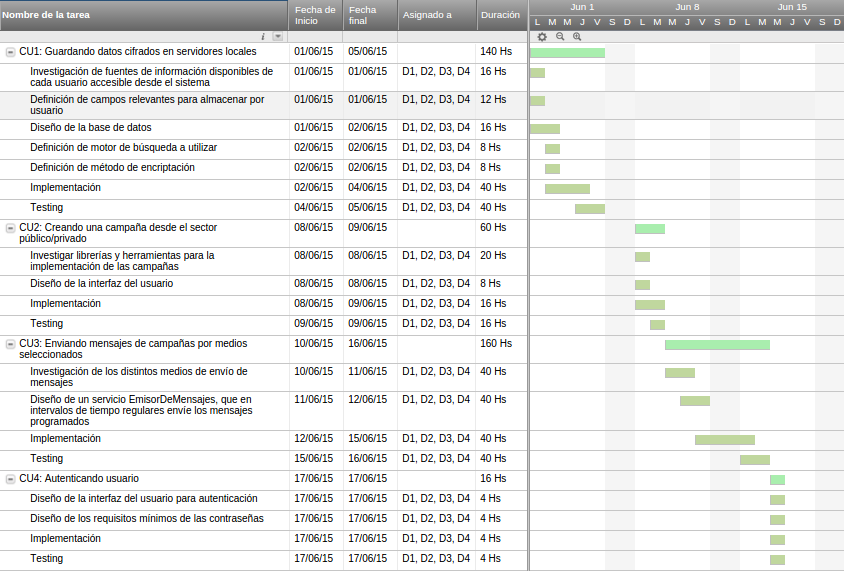
\includegraphics[width=1\textwidth]{gantt.png}
  \caption{Diagrama de Gantt de la 1era iteración con la asignación de tiempo}
  \label{fig:gantt}
\end{figure}

\newpage

%%%%%%%%%%%%%%%%%%%%%%%%%%%%%%%%%%%%%%%%%%%%%%%%%%%%%%%%%%%%%%%%%%%%%%%%%%%%%%%
%% Análisis de riesgo                                                        %%
%%%%%%%%%%%%%%%%%%%%%%%%%%%%%%%%%%%%%%%%%%%%%%%%%%%%%%%%%%%%%%%%%%%%%%%%%%%%%%%

\section{Análisis de riesgos}

\riesgo{1}
    {Mantener la disponibilidad del servicio en la totalidad del país es importante. Sin embargo, se conoce que la disponibilidad del servicio puede tener dificultades en algunas zonas, como por ejemplo la patagonia.}
    {Alta}
    {Alto}
    {Alta}
    {Mantener un sistema que permita verificar la conexión de los distintos nodos que se encuentran en distintas regiones del país}
    {Al reportarse un fallo en la conexión, tercerizar la conexión a privados hasta que se arregle el problema}

\riesgo{2}
    {ArSat nos provee actualmente conexión y procesamiento en la región de Córdoba. Si se encuentra un problema en los nodos de ANSES, existirán problemas para procesar la información almacenada.}
    {Media}
    {Medio}
    {Medio}
    {Realizar backups de los nodos regionales con cierta frecuencia y almacenarlos de forma cifrada en una empresa tercerizada; controlar el estado de los nodos dentro de las regiones}
    {Utilizar el backup cifrado en la empresa para solventar la baja del servidor mientras se arregla. Registrar las acciones realizadas mientras el nodo está caído y actualizarlas con la información fresca al arreglarse.}

\riesgo{3}
    {El modelo de abono que contabiliza los mensajes enviados está por migrar pronto a mejores servidores, por lo que se esperan algunas fallas de comunicación durante la transición.}
    {Alta}
    {Alto}
    {Alta}
    {Mantener un sistema de respaldo durante la migración del servicio para así poder asegurar la comunicación.}
    {Utilizar el sistema de respaldo para mantener la mayor correctitud posible los balances en el modelo de abonos a privados.}

\newpage

\section{Atributos de calidad}

Los atributos de calidad principales que debe respetar el sistema a realizar, en orden de prioridad, son los que siguen:

\begin{enumerate}
\item Disponibilidad
\item Performance
\item Seguridad
\item Certeza de Datos
\item Modificabilidad
\item Flexibilidad
\item Usabilidad
\end{enumerate}

Para describirlos, decidimos detallar escenarios correspondientes a cada uno de ellos:

\subsection{Disponibilidad}
\escenario{El sistema debe ser capaz de soportar fallas de los distintos enlaces de comunicación.}
    {Interna.}
    {Se produce una falla en la conexión.}
    {Operación degradada.}
    {Conexiones del sistema.}
    {Se cambia rápidamente a otro tipo de conexión.}
    {Se tarda a lo sumo 10 minutos en cambiar a otro enlace de comunicación.}


\subsection{Modificabilidad}
\escenario{Se quiere poder integrar todos los planes de salud a nivel nacional y provincial, y todo tipo plan de comunicación gubernamental.}
    {Interna.}
    {Se desea extender el sistema.}
    {Operación normal.}
    {Sistema.}
    {El sistema es modificable en el menor tiempo posible.}
    {La extensión planteada no toma más de 8hs hombre modificando módulos relacionados.}

\escenario{Se quiere poder agregar nuevas campañas en todo momento.}
    {Interna.}
    {Un usuario desea agregar una campaña en el sistema.}
    {Operación normal.}
    {Sistema.}
    {El sistema es extensible al agregado de campañas nuevas en cualquier momento.}
    {El sistema permite el agregado de una nueva campaña el 99.9\% de las veces.}


\subsection{Certeza de datos}
\escenario{Como el otorgamiento de información precisa en tiempo real es imposible (aún con el equipo necesario), se debe proveer datos estimados.}
    {Interna.}
    {Un usuario desea ver la evolución de una campaña.}
    {Operación normal.}
    {Sistema.}
    {Se presentan datos estimados de la campaña, lo más precisos posibles.}
    {Los datos presentados tienen una precisión del 98\% respecto del análisis en tiempo real.}

\subsection{Seguridad}

\escenario{Quiere asegurar confidencialidad de todos los datos involucrados.}
    {Externa.}
    {Un individuo malintencionado intenta interferir los mensajes que se envían entre enlaces.}
    {Online.}
    {Sistema.}
    {Se utilizan cifrados para los mensajes los cuales tardarían un tiempo alto en romperse sin las claves correspondientes.}
    {Se tarda más de 10 mil años en realizar la decodificación sin claves.}

\escenario{Sólo personal autorizado y sus delegados en cada provincia tengan acceso a definir las campañas, y evolución.}
    {Externa.}
    {Un usuario sin privilegios intenta acceder a datos sobre campañas o definir una.}
    {Online.}
    {Sistema.}
    {Se utiliza un sistema de privilegios y accesos con un bajo porcentaje de accesos sin autorización.}
    {En las auditorías de seguridad, se obtiene acceso sin autorización un menos del 3\% de las veces.}

\escenario{Todos los datos que se manejarán son sensibles, y debe protegerse su acceso.}
    {Externa.}
    {Un individuo malintencionado intenta acceder a los datos guardados en las regiones o en el sistema de abono de datos.}
    {Online.}
    {Sistema.}
    {Se utilizan cifrados para los datos almacenados que tardarían un tiempo alto en decodificarse sin las claves correspondientes.}
    {Se tarda más de 10 mil años en realizar la decodificación sin claves.}

\subsection{Performance}

\escenario{Se debe poder monitorear el estado de las campañas de manera ágil. No se deben admitir demoras de ningún tipo.}
    {Externa.}
    {Un usuario desea ver el estado de una campaña.}
    {Operación normal.}
    {Sistema.}
    {Se visualizan los datos de la campaña.}
    {El estado de una campaña se actualiza en menos de 10 segundos.}

\escenario{Se quiere que distintas empresas puedan tener acceso rápidamente a los datos de evaluación para mejorar los perfiles de marketing.}
    {Interna.}
    {Una empresa desea acceder a los datos de evaluación.}
    {Operación normal.}
    {Sistema.}
    {Las empresas pueden acceder con gran velocidad a los datos de evaluación.}
    {Las empresas acceden a lo sumo en 60 segundos a los datos de evaluación de los usuarios.}

\subsection{Usabilidad}

\escenario{Se quiere que el sistema sea fácil de usar para todos aquellos interesados en promover campañas de todo tipo.}
    {Interna.}
    {Un usuario desea poder utilizar fácilmente el sistema para crear campañas.}
    {Operación normal.}
    {Sistema.}
    {Los usuarios pueden utilizar fácilmente el sistema.}
    {Los usuarios tardan menos de 30 minutos en aprender a crear campañas en el sistema.}


\newpage
\section{Justificación de la arquitectura}
Para la realización de la arquitectura correspondiente al Sistema BigTiza se tuvieron en cuenta, principalmente, los atributos de calidad descritos anteriormente. 	

En lo que sigue, explicamos la arquitectura realizada:

\begin{itemize}

\item Utilizamos un repositorio de campañas para el almacenamiento cifrado de los datos y otro para el almacenamiento de campañas (los mensajes de cada una de éstas).

\item Utilizamos un repositorio de usuarios, donde se guardan los usuarios y las contraseñas de los mismos.

\item El repositorio de grupos de personas almacenan los números de las personas por su categoría (si son fumadores, si son deportistas, etc.).

\item El selector de conexión (cumpliendo el rol de un proxy) verifica si el sistema de Arsat está caído, en cuyo caso elige la opción de utilizar el sistema de abono para la comunicación entre nodos regionales.

\item El actuador recibe las peticiones web y las atiende.

\end{itemize}

\newpage
\section{Arquitectura TP1}

Para la arquitectura del TP1, nos basamos en el diagrama de clases realizado considerando las decisiones tomadas a lo largo de la elaboración del mismo.

\begin{itemize}
\item El \textit{Servidor web} representa a la interfaz que se le muestra al usuario cuando desea ingresar al sistema.
\item El \textit{receptor de peticiones web} se encarga del manejo de los pedidos realizados por los usuarios. Éstas pueden incluir información sobre las mediciones de eficacia, sobre el estado de las campañas, agregado o supresión de mensajes, etc.
\item El \textit{Autenticador} verifica el usuario y la contraseña ingresados por el usuario para otorgarle los permisos que le corresponden.
\item El \textit{Autenticador} recibe la información del \textit{Repositorio de credenciales}, quien almacena la información de los directivos y maestros.
\item El \textit{Repositorio de mensajes} almacena los mensajes de las campañas. Funciona como repositorio (cuando un mensaje debe ser enviado al emisor de mensajes) y como blackboard (cuando un usuario agrega un nuevo mensaje).
\item El \textit{Repositorio de eventos} tiene guardados los eventos de las campañas y tiene el mismo rol que el repositorio de mensajes.
\item El \textit{Emisor de mensajes} es el encargado de transmitir los mensajes en tiempo y hora junto con los destinatarios de los mismos al \textit{Servicio de SMS} para que éste los envíe.
\item Para la realización de esto último, el \textit{Repositorio de alumnos} (que incluye a los padres de los mismos) le provee los datos necesarios al \textit{Emisor de mensajes} para que se les envíe a los alumnos correspondientes.
\end{itemize}

El diagrama resultante es el siguiente:

\grafico{./diagramas/arquitecturaTP1.png}
\newpage
\section{Comparación y conclusiones}

\end{document}
